\section*{Problem 3}

Use MATLAB to compute the DFT of the signals in Problem 2. In order to increase your accuracy,
pad the signals with zeros (for example. if you want to plot an additional 10 points, 
then add 10 zeros).
For the signal in part c), compute the DFT for three cases: truncating the signal at 
N = 5, N = 10 and at N= 20. In each case, compare your answers to those found in 
Problem 1 by plotting the magnitude of both versus frequency.

\subsection*{Solution}

\zcodemat{sources/c4p3.m}{Comparison of results of DTFT vs DFT}

\begin{figure}[H]
\caption{Plot of DFT vs FDTD for points (a) and (b)}
\centering
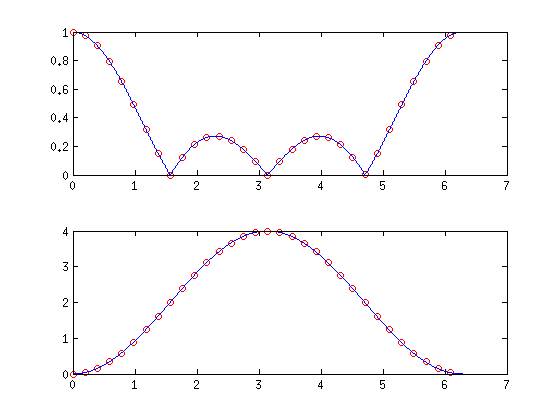
\includegraphics[width=0.8\textwidth]{figs/c4p32.png}
\label{fig:c4p31}
\end{figure} 

\begin{figure}[H]
\caption{Plot of DFT vs FDTD for point (c) and N=[5,10,20]}
\centering
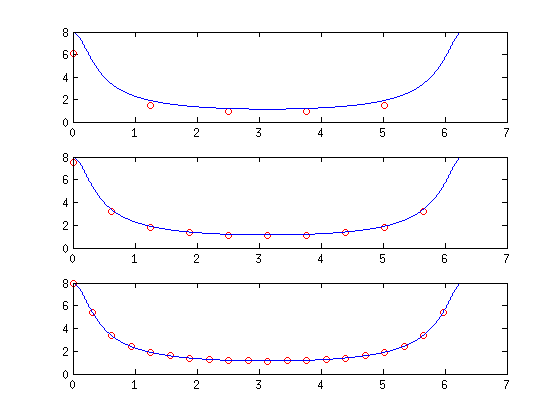
\includegraphics[width=0.8\textwidth]{figs/c4p31.png}
\label{fig:c4p32}
\end{figure} 

